%!TEX root = skripsi.tex
%-----------------------------------------------------------------------------%
\chapter{\babDua}
%-----------------------------------------------------------------------------%
Pada bab ini, dijelaskan mengenai studi literatur yang dilakukan. Studi literatur yang dilakukan digunakan sebagai dasar konsep dan teknik penelitian. Dipaparkan pula berbagai istilah dan metode yang digunakan dalam penelitian.


%-----------------------------------------------------------------------------%
\section{Leksikal Semantik}
%-----------------------------------------------------------------------------%
Dalam \textit{natural language processing}, terdapat beberapa tingkatan untuk merepresentasikan suatu informasi yaitu kata, sintak, dan semantik. Kata adalah kumpulan simbol yang memiliki arti (\textit{sense}) tertentu. Sintak berarti struktur dari kata yang bila digabung akan membentuk arti baru. Semenatara semantik berarti arti atau makna dari kata itu sendiri. Suatu kata tidak hanya mengandung makna namun juga relasi antar kata serta struktur internal. Studi yang mempelajari sistematik struktur serta relasi semantik disebut Leksikal Semantik \citep{jurafsky2000speech}. % TODO: ask this. Too faguee

Sebelum melangkah lebih lanjut, perlu diketahui beberapa istilah dasar dalam bidang ini. Kata dapat disebut sebagai lexeme yang mengandung suatu bentuk orthographic dan arti di dalamnya. Kumpulan lexeme tersimpan dalam lexicon atau dapat juga dikenal sebagai kamus. Arti dari suatu lexeme sebenarnya merupakan rangkaian lexeme lain yang mendeskripsikannya.

Bahasa Inggris memiliki kamus digital yang menyimpan segala informasi kata dan strukturnya yang disebut WordNet\footnote{wordnet.princeton.edu}. WordNet tersebut sering digunakan untuk menunjang berbagai penelitian di bidang \textit{natural language processing}. 

%-----------------------------------------------------------------------------%
\subsection{Word Features}
%-----------------------------------------------------------------------------%
Suatu kata dapat dilihat dari berbagai bentuk, seperti bentuk orthographic dan phonemic-nya. Suatu kata juga memiliki arti (\textit{sense}) yang merepresentasikan deskripsi terhadap kata tersebut. Sayangnya, bentuk-bentuk tersebut tidak dapat dengan mudah diproses oleh komputer. Melalui berbagai penelitian yang telah dilakukan sebelumnya, kata dapat direpresentasikan ke dalam bentuk yang dapat dibaca oleh mesin. Berikut adalah beberapa perbandingan bentuk representasi kata yang bisa dibaca oleh mesin dan manusia.

%-----------------------------------------------------------------------------%
\subsubsection{Orthographic}
%-----------------------------------------------------------------------------%
Orthographic adalah bentuk paling dasar dari suatu kata. Bentuk ini merepresentasikan rangkaian simbol-simbol yang tersusun membentuk suatu kata yang memiliki arti. Studi mengenai bentuk ini banyak digunakan untuk mengetahui perbandingan bentuk kata dasar dengan kata berimbuhan. Bentuk phonemic adalah bagaimana kata tersebut dilafakan. Karena penelitian ini hanya berfokus pada teks, maka hanya diperhatikan bentuk orthographic suatu kata.

%-----------------------------------------------------------------------------%
\subsubsection{Sense}
%-----------------------------------------------------------------------------%
Sense adalah makna dari kata tersebut atau definisi kata. Informasi mengenai makna kata disimpan dalam kamus bahasa tersebut. Dalam kamus (lexicon), sense terbentuk dari lexeme-lexeme lain yang mendeskripsikan lexeme tersebut. 

%-----------------------------------------------------------------------------%
\subsubsection{Word Embedding}
%-----------------------------------------------------------------------------%
\textit{Word Embedding} digunakan untuk menentukan similarity antar kata relasi yang dihasilkan dari proses \textit{Pattern Matching}.

%-----------------------------------------------------------------------------%
\subsubsection{POS Tag}
%-----------------------------------------------------------------------------%
Part-of-speech tagging adalah proses mengelompokan setiap kata dalam suatu kalimat ke dalam kategori yang bersesuaian.  

%-----------------------------------------------------------------------------%
\subsection{Relasi Kata}
%-----------------------------------------------------------------------------%
Sebelum membahas lebih lanjut mengenai relasi kata, perlu diketahui apa itu relasi. Relasi menggambarkan hubungan atau koneksi yang dimiliki oleh suatu hal dengan yang lain (KBBI). Dalam bidang matematika, relasi memetakan suatu anggota dari himpunan satu ke himpunan lain sesuai dengan hubungan yang didefinisikan. Dalam penelitian ini, relasi yang diperhatikan adalah relasi kata yang berarti satu kata akan dipetakan ke dalam kata lain. Domain untuk kata tersebut adalah kata benda (\textit{noun}) dalam Bahasa Indonesia.

Satu relasi dapat terdiri dari beberapa entitas dan dituliskan dalam bentuk tuple $t = (e_1, e_2, ..., e_n)$ dimana $e_i$ adalah suatu entitas yang memiliki relasi $r$ dalam dokumen $D$ \citep{bach2007review}. Relasi sinonim dapat ditulis dalam notasi tersebut. Selain relasi yang mengandung beberapa entitasi, banyak relasi yang hanya menghubungkan antar dua entitas (relasi biner), seperti \textit{terletak-di(Universitas Indonesia, Depok)} atau \textit{ditulis-oleh(Habis Gelap Terbitlah Terang, RA Kartini)}. Relasi kata sendiri dapat didefinisikan secara bebas seperti contoh sebelumnya maupun merupakan relasi khusus seperti relasi semantik.

Semantik adalah arti (\textit{sense}) dari suatu kata. Relasi semantik kata adalah hubungan yang dimiliki antar kata berdasarkan arti atau makna dari kata tersebut. Beberapa relasi semantik adalah sebagai berikut \citep{miller1995wordnet}.
\begin{itemize}
  \item Sinonim adalah relasi antar kata dimana dua kata yang berbeda memiliki arti yang sama. Semua kelas kata dapat memiliki relasi sinonim. Dalam WordNet, relasi ini direpresentasikan dalam bentuk \textit{synset} dan bersifat simetris. Sebagai contoh 'makan', 'melahap', dan 'menyantap' memiliki makna yang sama.
  \item Antonim adalah yang menggambarkan arti yang saling berkebalikan antar kata. Umumnya relasi ini digunakan pada kelas kata sifat (\textit{adverb}) dan kata keterangan (\textit{adjective}). Sama seperti synonymy, relasi ini memiliki sifat simetris. Sebagai contoh kata 'tinggi' memiliki makna yang berkebalikan dengan kata 'pendek'.
  \item Hiponim adalah relasi yang menyatakan hubungan kata yang lebih khusus. Sementara untuk kata yang lebih umum dikenal dengan relasi hipernim. Kedua relasi ini diperuntukan kelas kata benda (\textit{noun}) dan umumnya satu kata memiliki hanya satu hipernim. Kedua relasi ini bersifat transitif, sehingga dapat digambarkan dalam bentuk hirarki. Sebagai contoh kucing, ikan, kelinci (hiponim) adalah binatang (hipernim). Binatang adalah hiponim dari makhluk hidup. Sehingga dapat dikatakan pula bahwa kucing, ikan, kelinci (hiponim) adalah makhluk hidup (hipernim).
  \item Meronim dan holonim adalah relasi yang menyatakan hubungan bagian satu dengan yang lain, dimana meronim menyatakan sub-bagian dan holonim menyatakan bagian yang lebih besar. Seperti relasi hyponym-hypernym, relasi meronim-holonim bersifat transitif dan dapat digambarkan dalam bentuk hirarki. Dalam WordNet, relasi ini dibagi ke dalam tiga bagian yaitu \textit{part-meronym}, \textit{member-meronym}, dan \textit{substance-meronym}. Sebagai contoh sebuah sel (holonim) memiliki nukleus, ribosom, mitokondria (meronim).
  \item \textit{Troponymy} adalah relasi seperti hiponim-hipernim yang khusus untuk kelas kata kerja (\textit{verb}). Dalam Bahasa Inggris, contoh kata yang memiliki relasi ini adalah 'stroll' dan 'walk'.
\end{itemize}


%-----------------------------------------------------------------------------%
\section{Leksikal Semantik Resources}
%-----------------------------------------------------------------------------%
Kebutuhan menyimpan suatu korpus yang merupakan leksikal semantik resource. Informasi mengenai kata, makna, serta relasi di dalamnya tersebut perlu tersimpan secara baik sehingga dapat digunakan. Informasi tersebut juga perlu disimpan sedemikian sehingga dapat dapat dibaca mesin dan digunakan untuk proses komputasi. Bahasa Inggris telah membuat kamus digital yaitu WordNet yang banyak digunakan untuk berbagai penelitian. Sementara untuk Bahasa Indonesia, penelitian yang berusaha membangun WordNet telah dilakukan sebelumnya, namun masih ditemukan beberapa kekurangan dari WordNet Bahasa yang ada. 

%-----------------------------------------------------------------------------%
\subsection{WordNet}
%-----------------------------------------------------------------------------%
WordNet adalah kamus leksikal yang tersimpan secara digital dan digunakan untuk berbagai keperluan komputasi \citep{miller1995wordnet}. Pembuatan WordNet dilatarbelakangi keperluan mendapatkan \textit{sense} atau arti semantik suatu kata. Informasi tersebut perlu disimpan dan dapat dibaca oleh mesin. WordNet pertama dibuat oleh \cite{miller1995wordnet} berbasis Bahasa Inggris dan sekarang dikenal dengan nama Princeton WordNet (PWN). WordNet menyimpan informasi dalam bentuk database dimana setiap entry-nya adalah pasangan \textit{synset} dan arti semantiknya (\textit{sense}). Set sinonim (\textit{synset}) adalah himpunan kata yang memiliki arti yang sama atau saling berelasi \textit{synonym}. 

Kata dalam WordNet dikelompokkan ke dalam beberapa kelas kata yaitu kata benda (\textit{noun}), kata kerja (\textit{verb}), kata sifat (\textit{adjective}), dan kata keterangan (\textit{adverb}). WordNet juga menyimpan informasi mengenai relasi semantik antar \textit{synset}. Relasi yang disimpan adalah sinonim, \textit{antonymy}, hiponim, hipernim, \textit{meronymy}, \textit{holonymy}, \textit{troponymy}, dan \textit{entailment}. Hingga penulisan ini, versi WordNet yang sudah ada adalah versi 3.1 yang dapat diakses melalui situs resminya maupun diunduh datanya. Sementara aplikasi yang sudah terintegrasi dengan sistem UNIX/Linux adalah versi 3.0. 

Penelitian mengenai WordNet Bahasa Indonesia pernah dilakukan sebelumnya oleh \cite{putra2008building} serta \cite{margaretha2008comparing}. Indonesian WordNet (IWN) dibangun menggunakan metode mapping antara WordNet yang sudah ada ke dalam Bahasa Indonesia \citep{putra2008building}. WordNet yang digunakan sebagai dasarnya adalah Princeton WordNet. Synset dalam PWN akan dipetakan ke dalam \textit{entry} Kamus Besar Bahasa Indonesia (KBBI), sehingga menghasilkan hasil yang berkualitas baik secara cepat dan mudah. Penelitian tersebut menghasilkan 1441 synset dan 3074 sense. Relasi semantik antar synset diperoleh dengan memetakan IWN synset dengan PWN synset, sehingga relasi yang dimiliki dalam PWN dapat diturunkan.

Pengembangan WordNet untuk Bahasa Indonesia juga dilakukan oleh Nanyang Technology University (NTU) sejak tahun 2011 dan diberi nama WordNet Bahasa \citep{noor2011creating}. WordNet ini telah diintegrasi dengan salah satu \textit{tools} NLP berbasis Python yaitu nltk sehingga dapat dengan mudah digunakan dalam komputasi. WordNet Bahasa juga memanfaatkan PWN untuk mendapatkan relasi semantik antar \textit{synset}. Pada penelitian ini, dimanfaatkan \textit{tools} tersebut untuk mendapatkan \textit{seed} relasi semantik antar kata dalam Bahasa Indonesia.

Walau beberapa penelitian sudah dilakukan sebelumnya, WordNet Bahasa Indonesia masih memiliki beberapa kekurangan. Jumlah kata yang terkandung di dalamnya masih terbatas. Sementara itu, relasi semantik antar kata yang dimiliki oleh WordNet Bahasa Indonesia merupakan hasil turunan dari relasi semantik WordNet Princeton. Hal ini menyebabkan ketergantungan untuk mendapatkan relasi semantik dengan struktur dari PWN. Selain itu, beberapa \textit{synset} Bahasa Indonesia juga tidak dapat dipetakan secara tepat ke \textit{synset} PWN yang menyebabkan beberapa kata kehilangan arti atau mendapat arti yang kurang tepat. Jika berusaha dibentuk ke dalam relasi biner, pasangan kata relasi semantik Bahasa Indonesia yang dihasilkan terlihat kurang baik. Untuk itu, dicetuskanlah penelitian untuk mengekstrak relasi semantik dalam Bahasa Indonesia secara mandiri. 


%-----------------------------------------------------------------------------%
\section{Relation Extraction}
%-----------------------------------------------------------------------------%
\textit{Relation extraction} adalah cabang dari \textit{Information Extraction} (IE) yang berfokus pada proses ekstraksi relasi antar kata. Proses ini berusaha mengekstrak informasi terstruktur dengan definisi yang diinginkan dari teks dokumen atau resource yang tidak terstruktur. Beberapa contoh penelitian ini seperti \textit{named entity recognition} (NER) yang mengetahui apakah suatu entitas adalah orang, organisasi, atau lokasi \citep{bikel1999algorithm}. 

%-----------------------------------------------------------------------------%
\subsection{Semantic Relation Extraction}
%-----------------------------------------------------------------------------%
\textit{Semantic relation extraction} mengkhususkan pada proses ekstraksi relasi semantik antar kata. Penelitian dalam bidang ini sudah banyak dilakukan dengan berbagai metode. Salah satu metode populer untuk mendapatkan relasi semantik satu domain bahasa adalah menggunakan \textit{pattern extraction} dan \textit{pattern matching} seperti yang telah dilakukan pada penelitian \cite{hearst1992automatic}, \cite{ruiz2005automatic}, dan \cite{arnold2014extracting}. Penelitian lain memanfaatkan distribusi kata untuk memperoleh \textit{semantic distance} antar kata. \textit{Semantic distance} adalah nilai yang merepresentasikan kedekatan antar kata berdasarkan semantiknya.

Penelitian yang dilakukan oleh \cite{hearst1992automatic} merupakan salah satu penelitian awal ekstraksi relasi semantik yang menggunakan metode \textit{pattern extraction} dan \textit{matching}. Hearst menggunakan \textit{lexico-syntactic pattern} untuk mendapatkan pasangan kata relasi tanpa membutuhkan pengetahuan sebelumnya dan dapat diaplikasikan dalam teks apapun. Pada awal, Hearst mendifiniskan dua \textit{pattern} berdasarkan hasil observasi dari teks. Selanjutnya, \textit{pattern} baru didapat menggunakan langkah berikut. 
\begin{enumerate}
  \item Tentukan relasi yang akan diamati dan kumpulkan entitas yang menggambarkan relasi tersebut.
  \item Dalam teks dokumen, cari lokasi dimana entitas-entitas tersebut berada dan simpan kata-kata diantaranya (lingkungan).
  \item Cari kesamaan dari teks yang terekstraksi dan bentuk suatu \textit{pattern} baru.
  \item Jika \textit{pattern} baru telah terbukti benar, gunakan \textit{pattern} tersebut untuk mendapatkan entitas baru.
\end{enumerate}
Proses evaluasi dilakukan dengan membandingkan entitas yang dihasilkan dengan synset dalam WordNet. 

Penelitian yang dilakukan oleh \cite{ruiz2005automatic}, memanfaatkan WordNet dan Wikipedia sebagai korpus untuk mendapatkan pasangan kata relasi. Pertama dilakukan \textit{entry sense disambiguation} yang merupakan tahap \textit{pre-processing} untuk memetakan setiap entri dalam Wikipedia dengan \textit{synset} dalam WordNet. Tahap berikutnya adalah ekstraksi \textit{pattern} antara dua konsep. Jika terdapat dua konsep yang saling berhubungan dan memiliki suatu relasi semantik dalam WordNet maka kalimat yang mengandung dua konsep tersebut akan disimpan. Proses tersebut menghasilkan daftar relasi semantik dengan masing-masing memiliki \textit{pattern} di dalamnya. Dari banyak \textit{pattern} yang dihasilkan, proses selanjutnya adalah \textit{pattern generalisation} yang bertujuan membuat pattern yang lebih umum. Tahap ini memanfaatkan algoritma \textit{edit-distance} dengan modifikasi. Setelah mendapatkan \textit{pattern}, tahapan terakhir adalah menggunakannya ke dalam korpus untuk mendapatkan entitas baru.

Penelitian yang dilakukan \cite{arnold2014extracting} juga memanfaatkan korpus Wikipedia dan menggunakan \textit{pattern}. Selain \textit{hypernym-hyponymy} dan \textit{holonym-meronymy}, penelitian ini juga mengidentifikasi relasi sinonim. Kalimat definisi pada Wikipedia di-\textit{parse} menggunakan \textit{Finite State Machine} (FSM) dan konsep-konsep baru diekstrak menggunakan \textit{pattern} yang telah didefinisikan. Penelitian lain yang dilakukan oleh \cite{sumida2008hacking} memanfaatkan struktur internal Wikipedia dalam mengekstraksi \textit{pattern} relasi untuk Bahasa Jepang. 


%-----------------------------------------------------------------------------%
\section{Korpus}
%-----------------------------------------------------------------------------%
Korpus adalah data yang dengan format yang dapat dibaca oleh mesin dan memiliki fungsi spesifik \citep{atkins1992corpus}.

%-----------------------------------------------------------------------------%
\subsection{Korpus Pasangan Kata Relasi Semantik}
%-----------------------------------------------------------------------------%
Saat ini, belum ada korpus independen yang menggambarkan relasi semantik antar kata dalam Bahasa Indonesia. Relasi semantik Bahasa Indonesia yang ada saat ini didapatkan dari hasil relasi turunan pemetaan \textit{synset} Bahasa Indonesia dengan PWN. 

Korpus relasi semantik yang ingin dibuat menyimpan informasi dalam bentuk pasangan kata yang berelasi serta relasi yang menghubungkannya. Selanjutnya, pasangan kata berelasi akan disebut sebuah \textit{pair}. Untuk relasi yang bersifat transitif seperti \textit{hypernym-hyponym}, ada identifikasi kata mana yang merupakan hipernim dan mana yang merupakan hiponim. Relasi hipernim dan hiponim adalah relasi bersifat transitif yang dapat direpresentasikan dalam bentuk hirarki. Pada penelitian ini, korpus \textit{pair} yang diperoleh merepresentasikan hubungan yang berjarak tepat satu dari yang lain. 


%-----------------------------------------------------------------------------%
\section{Wikipedia}
%-----------------------------------------------------------------------------%
Wikipedia\footnote{www.wikipedia.org} adalah ensiklopedia terbuka yang memuat berbagai bahasa dan merupakan hasil kolaborasi berbagai penulis \citep{denoyer2006wikipedia}. Wikipedia adalah salah satu korpus teks dokumen terbesar yang disimpan secara \textit{online} yang dapat diakses dan diunduh secara bebas. Wikipedia dikelola oleh organisasi nonprofit bernama Wikimedia Foundation. Pada tahun 2009, jumlah kontributor Wikipedia Bahasa Indonesia telah mencapai 2.502 pengguna aktif. Walau ditulis oleh berbagai narasumber, informasi yang dimuat dalam Wikipedia dibuat secara terstruktur dengan bahasa yang formal. Wikipedia juga memuat informasi umum terbaru \citep{arnold2014extracting}.

%-----------------------------------------------------------------------------%
\subsection{Korpus Wikipedia}
%-----------------------------------------------------------------------------%
Wikipedia Bahasa Indonesia saat ini telah memuat lebih dari 400.000 artikel dari berbagai domain. Artikel-artikel yang disimpan dalam Wikipedia dapat diunduh secara gratis dalam bentuk \textit{dumps}\footnote{dumps.wikimedia.org} dengan format XML. Beberapa tipe \textit{dump} dapat dipilih, diantarnya adalah halaman seluruh artikel, halaman artikel beserta \textit{revision history}, daftar judul artikel, dan lainnya. Secara berkala, Wikimedia membuat \textit{dump} terhadap seluruh artikel terakhir yang disimpan untuk setiap bahasa. Pada situs yang menyediakan pengunduhan data Wikipedia, terdapat tanggal unik yang menyatakan tanggal terakhir data tersebut di-\textit{update}.

%-----------------------------------------------------------------------------%
\subsection{Wikipedia sebagai Lexical Semantic Resource}
%-----------------------------------------------------------------------------%
Artikel dalam Wikipedia terdiri dari berbagai domain kategori dan memuat berbagai \textit{noun} umum. Walau ditulis secara kolaboratif, Wikipedia memuat artikel secara terstruktur dimana pada paragraf pertama umumnya berisi kalimat-kalimat definisi menganai topik yang sedang dibahas. Bahasa yang ditulis juga cukup formal dan terstruktur. Selain itu, sudah banyak penelitian ekstraksi relasi semantik dengan metode pattern yang menggunakan artikel Wikipedia seperti penelitian \cite{ruiz2005automatic} dan \cite{arnold2014extracting}. 

%-----------------------------------------------------------------------------%
%-----------------------------------------------------------------------------%
\section{Pattern}
%-----------------------------------------------------------------------------%
\textit{Pattern} adalah suatu bentuk yang dapat merepresentasikan kumpulan data berukuran besar. Pada teks dokumen, \textit{pattern} dapat terbentuk secara eksplisit ataupun implisit. Secara eksplisit seperti \textit{lexico-syntactic pattern} yang terbentuk dari kata-kata di dalam dokumen tersebut. Sementara \textit{pattern} terbentuk secara implisit jika dilhat dari kemiripan vektor yang merepresentasika dokumen atau kata-kata di dalam dokumen tersebut.

%-----------------------------------------------------------------------------%
\subsection{Lexico-syntactic Pattern}
%-----------------------------------------------------------------------------% 
\textit{Lexico-syntactic pattern} adalah \textit{pattern} yang hanya memanfatkan kata-kata dalam korpus dokumen dan dimanfaatkan untuk proses \textit{string matching}. Salah satu \textit{pattern} leksikal yang terkenal adalah Hearst Pattern yang merepresentasikan pola-pola untuk mendapatkan relasi hiponim dari dokumen \citep{hearst1992automatic}. Menurut Hearst, beberapa syarat yang harus dipenuhi suatu \textit{lexico-syntactic pattern} yang baik adalah sebagai berikut.
\begin{itemize}
  \item Kemunculannya sering pada teks dalam berbagai domain sehingga dapat mengekstrak banyak entitas.
  \item Merepresentasikan relasi yang diinginkan sehingga hasil ekstraksi juga benar.
  \item Dapat dikenali tanpa membutuhkan pengetahuan sebelumnya sehingga dapat dibentuk dalam situasi apapun.
\end{itemize}

%-----------------------------------------------------------------------------%
%-----------------------------------------------------------------------------%
\section{Pattern Extraction dan Matching}
%-----------------------------------------------------------------------------%
\textit{Pattern extraction} atau \textit{pattern recognition} adalah salah satu cabang dalam \textit{machine learning} yang berusaha mencari pola kemiripan tertentu dari kumpulan data yang diberikan. \textit{Pattern matching} adalah proses untuk mencocokkan suatu \textit{pattern} dengan kumpulan data yang belum dianotasi. Penelitian ekstraksi relsasi semantik menggunakan metode pattern matching telah dilakukan oleh \cite{hearst1992automatic}, \cite{ruiz2005automatic}, \cite{arnold2014extracting}, dan \cite{sumida2008hacking}.

Banyaknya penelitian menggunakan metode \textit{pattern matching} dan \textit{extraction} menjadi salah satu alasan penggunaan metode tersebut untuk mengekstrak relasi kata dalam Bahasa Indonesia. Pada penelitian ini, relasi semantik yang diekstrak dibatasi hanya untuk relasi \textit{hypernym-hyponym}. 


%-----------------------------------------------------------------------------%
%-----------------------------------------------------------------------------%
\section{Sequence Analyisis}
%-----------------------------------------------------------------------------%
Dalam bidang bioinformatik, \textit{suquence analysis} digunakan untuk mengetahui apakah suatu DNA atau RNA mengandung \textit{sequnce} tertentu. Pada penelitian ini, \textit{pattern} yang dihasilkan adalah \textit{pattern} leksikal yang merupakan deretan kata-kata. Algoritma seperti \textit{standard trie} dan \textit{suffix tree} dimanfaatkan secara berurut untuk proses \textit{pattern extraction} dan \textit{matching}.

%-----------------------------------------------------------------------------%
\subsection{Standard Trie}
%-----------------------------------------------------------------------------% 
\textit{Standard Trie} untuk suatu himpunan \textit{string} $S$ adalah \textit{ordered tree} dengan ketentuan berikut.
\begin{itemize}
  \item Setiap \textit{node}, selain \textit{root}, diberi label sebuah \textit{character}
  \item \textit{Children} dari sebuah \textit{node} terurut sesuai alphabet
  \item \textit{Path} dari eksternal \textit{node} hingga \textit{root} membentuk suatu \textit{string} dalam $S$.
\end{itemize}
\textit{Standard Trie} membutuhkan memori sebesar $O(n)$ dimana $n$ adalah total ukuran \textit{string} dalam $S$. Operasi \textit{insert} membutuh waktu $O(dm)$ dimana $m$ adalah ukuran \textit{string} yang baru dan $d$ adalah ukuran alphabet.

Sebagai contoh berikut adalah \textit{standard trie} yang dibangun dari himpunan \textit{string} {apel, ayam, baju, baja, bara}.
\begin{figure}
    \centering
    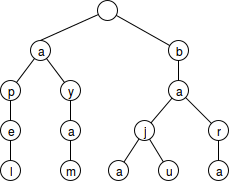
\includegraphics[scale=0.6]{pics/Contoh-StandardTrie}
    \caption{Contoh Standard Trie}
    \label{fig:contoh-standard-trie}
\end{figure}

%-----------------------------------------------------------------------------%
\subsection{Suffix Tree}
%-----------------------------------------------------------------------------% 
\textit{Suffix tree} sering digunakan untuk pencarian sequence yang panjang seperti \textit{genomes} untuk bidang bioinformatik. Pembentukan \textit{suffix tree} mirip seperti \textit{Standard Trie}, namun untuk seluruh \textit{suffix} dalam \textit{string}. Jika diberikan \textit{string} dengan panjang $n$, dibentuk cabang dengan $n(n-1)/2$ \textit{suffix}.  Metode ini banyak dimanfaatkan untuk mempercepat proses pencarian jika diberikan sebuah masukan \textit{query}. Jika terdapat sebuah \textit{pattern} dengan panjang \textit{string} $m$, maka waktu yang dibutuhkan untuk menjalankan proses \textit{pattern matching} adalah $O(dm)$ dengan $d$ adalah ukuran alfabet. Proses pencarian dilakukan dengan menelusuri \textit{path} dari \textit{root} sesuai dengan \textit{sequence query}. Jika seluruh karakter dalam \textit{query} selesai dijalankan, maka proses pencarian berhasil. 

Sebagai contoh \textit{string} 'babaa' menghasilkan \textit{suffix tree} berikut. Jika diberi \textit{query} 'ba' maka akan berhasil terhadap \textit{path} 'babaa' dan 'baa'.
\begin{figure}
    \centering
    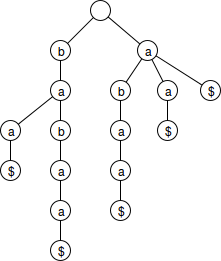
\includegraphics[scale=0.6]{pics/Contoh-SuffixTree}
    \caption{Contoh Suffix Trie}
    \label{fig:contoh-suffix-trie}
\end{figure}

%-----------------------------------------------------------------------------%
%-----------------------------------------------------------------------------%
\section{Semi Supervised}
%-----------------------------------------------------------------------------%
Dalam \textit{machine learning} terdapat dua tipe pendekatan yang umum digunakan yaitu \textit{supervised} dan \textit{unsupervised learning}. Supervised menggunakan data berlabel sebagai data \textit{training} maupun \textit{testing}. Dari kedua data tersebut, dibentuk suatu \textit{classifier} yang dapat memenuhi segala kasus yang mungkin terjadi. Data \textit{testing} digunakan untuk menguji kebaikan \textit{classifier} yang terbentuk. \textit{Unsupervised} menggunakan data yang tidak diberi label sama sekali dan berusaha untuk menemukan pola yang sama untuk suatu kumpulan data tertentu \citep{prakash2014survey}. Pendekatan lain yang merupakan kombinasi antara \textit{supervised} dan \textit{unsupervised learning} adalah \textit{semi supervised learning}. 

\textit{Semi supervised} adalah pendekatan \textit{machine learning} dimana informasi \textit{supervised} data diberikan tidak untuk seluruh data. Sebagian data merupakan data berlabel sementara sebagian lainnya belum memiliki label. Beberapa metode penerapan semi supervised adalah \textit{bootstrapping} (\textit{self training}), \textit{mixture models}, \textit{graph based methods}, \textit{co-training,} dan \textit{multiview learning}.
%(12) MITPress - Semi Supervised Learning

%-----------------------------------------------------------------------------%
\subsection{Bootstrapping}
%-----------------------------------------------------------------------------% 
Model \textit{bootstrapping} merupakan salah satu model \textit{semi supervised learning} yang paling umum digunakan. \textit{Bootstrapping} menggunakan data berlabel berukuran kecil dan data tidak berlabel berukuran jauh lebih besar. Proses anotasi data tidak berlabel dilakukan secara bertahap melalui sejumlah iterasi. Dari data \textit{training} berlabel, dibentuk suatu \textit{classifier} yang kemudian digunakan untuk menganotasi data tidak berlabel. Sejumlah $k$ data baru yang merupakan hasil pelabelan, dimasukkan ke dalam kelompok data berlabel. Proses tersebut dilakukan secara berulang, sehingga semakin lama iterasi jumlah data berlabel akan bertambah. 

Terdapat dua algoritma \textit{bootstrapping} yang pernah digunakan untuk proses \textit{pattern extraction} dan \textit{matching} yaitu \textit{Meta-Bootstrapping} dan \textit{Basilisk} \citep{riloff2003learning}. Keduanya digunakan untuk mengelompokan kata ke dalam suatu kategori semantik jika diberikan korpus teks yang belum dianotasi dan suatu \textit{seed}. \textit{Seed} didefinisikan sebagai korpus kata yang sudah diketahui kategori semantiknya. Secara umum, proses ini akan mencari \textit{pattern} berdasarkan seed yang diberikan. Dari \textit{pattern} yang dihasilkan dan teks yang belum dianotasi, diekstrak entitas baru dan dikelompokan berdasarkan kategori semantiknya. Kata-kata tersebut akan digabungkan ke dalam korpus pasangan kata berelasi.

%-----------------------------------------------------------------------------%
\subsection{Meta Bootstrapping}
%-----------------------------------------------------------------------------% 
Berikut adalah beberapa proses \citep{riloff1999learning} yang dijalankan algoritma \textit{meta bootstrapping} jika diberikan \textit{seed} berukuran kecil yang berasal dari suatu kategori semantik dan korpus yang belum dianotasi.
\begin{enumerate}
  \item Mengekstraksi \textit{pattern} secara otomatis dengan menerapkan syntactic template.
  \item Untuk setiap \textit{pattern} akan diberi bobot berdasarkan jumlah seed yang menghasilkan \textit{pattern}.
  \item Diambil \textit{pattern} terbaik dan seluruh seed lama yang merepresentasikan \textit{pattern} maupun \textit{seed} baru yang berhasil diekstrak disimpan.
  \item Dilakukan pembobotan ulang untuk setiap \textit{pattern} menggunakan \textit{seed} lama dan baru.
\end{enumerate}
Proses diatas dinamakan \textit{mutual bootstrapping} dan setelah proses tersebut selesai, semua entitas baru hasil ekstraksi dievaluasi. Pembobotan entitas baru diberikan berdasarkan jumlah \textit{pattern} yang mengekstrak kata tersebut. Lima kata terbaik diterima dan dimasukkan ke kamus (korpus) kata berelasi untuk selanjutnya diproses ulang.

%-----------------------------------------------------------------------------%
\subsection{Basilisk}
%-----------------------------------------------------------------------------% 
Algoritma \textit{Basilisk} \citep{thelen2002bootstrapping} juga memanfaatkan \textit{pattern} dan \textit{seed} dalam membangun korpus untuk suatu kategori semantik tertentu. Beberapa tahapan yang dijalankan adalah sebagai berikut.
\begin{enumerate}
  \item Secara otomatis membentuk \textit{pattern} dan memberi bobot berdasarkan jumlah seed yang menghasilkan \textit{pattern}. Pattern terbaik dimasukan ke dalam \textit{Pattern Pool}.
  \item Untuk setiap entitas baru yang terekstraksi dari \textit{pattern}, dimasukan ke dalam \textit{Candidate Word Pool}. Pemberian bobot dilakukan berdasarkan jumlah \textit{pattern} yang mengekstraksi dan asosiasi kumulatif kata dengan \textit{seed}.
  \item Sepuluh kata terbaik diambil dan dimasukan ke dalam kamus (korpus) yang kemudian digunakan untuk iterasi selanjutnya. 
\end{enumerate}

Kateogori semantik untuk proses ini bisa lebih dari satu. \textit{Basilisk} memberi bobot berdasarkan informasi kolektif dari kumpulan \textit{pattern} yang mengekstrak kata tersebut. Sementara \textit{Meta-Bootstrapping} hanya mengambil satu \textit{pattern} terbaik dan mengelompokkan seluruh kata yang terekstrak dari \textit{pattern} ke dalam kategori semantik yang sama. Dari hasil penelitian komparatif yang pernah dilakukan \citep{riloff2003learning}, didapatkan \textit{Basilisk} mengungguli performa \textit{Meta-Bootstrapping}. 

%-----------------------------------------------------------------------------%
%-----------------------------------------------------------------------------%
\section{Pointwise Mutual Information}
%-----------------------------------------------------------------------------%
\textit{Pointwise Mutual Information} (PMI) adalah pengukuran nilai asosiasi antar variabel. Dalam bidang \textit{information theory}, PMI dapat dimanfaatkan untuk menghitung asosiasi kemunculan dua buah kata. Jika diberikan dua buah kata $x$ dan $y$, maka nilai PMI kata tersebut dalam suatu dokumen dapat dihitung menggunakan rumus berikut. 
\[ pmi(x;y)=log\frac{p(x,y)}{(x)p(y)}=log\frac{p(x|y)}{p(x)}=log\frac{p(y|x)}{p(y)} \] dengan $p(x)=\frac{f(x)}{N}$
\[ pmi(x;y)=log\frac{f(x)N}{f(x)f(y)} \]
\begin{itemize}
  \item $p(x)$ adalah probabilitas kemunculan kata $x$ dalam korpus
  \item $f(x)$ adalah frekuensi kemunculan kata $x$ dalam korpus
  \item $N$ adalah toatal seluruh kata dalam korpus
\end{itemize}
Pengukuran ini bersifat simetris, sehingga $p(x;y)=p(y;x)$. Nilai PMI dapat merupakan bilangan positif maupun negatif. Jika nilai PMI adalah nol (0), berarti kedua variabel saling \textit{independent}.

%-----------------------------------------------------------------------------%
\subsection{Skip PMI}
%-----------------------------------------------------------------------------% 
PMI umumnya hanya menggunakan model \textit{bigram} atau \textit{trigram}. Model ini hanya melihat hubungan kata yang berdampingan. Sebagai contoh ingin diketahui PMI untuk \textit{bigram} 'hong kong', 'sepak bola', dan 'amerika serikat'. Pada penelitian ini dilakukan modifikasi yaitu membuat model \textit{skip-gram} PMI. Kita menghitung nilai PMI antar dua kata yang dipisahkan dengan $n$ diantaranya. 

%-----------------------------------------------------------------------------%
%-----------------------------------------------------------------------------%
\section{Evaluasi}
%-----------------------------------------------------------------------------%
Evaluasi dilakukan untuk mengetahui kebaikan hasil penelitian. Evaluasi dapat dilakukan dengan mengukur akurasi data yang dihasilkan. Akurasi adalah nilai perbandingan antara jumlah data yang benar dengan jumlah seluruh data (Manning). 
\[ akurasi=\frac{jumlah\,\,data\,\,benar}{jumlah\,\,seluruh\,\,data} \]
Selain menghitung akurasi, proses evaluasi juga menghitung nilai-nilai lainnya. Berikut ada beberapa metode dan teknik evaluasi lain yang digunakan dalam penelitian.

%-----------------------------------------------------------------------------%
\subsection{Sampling}
%-----------------------------------------------------------------------------% 
Terdapat dua kategori utama dalam \textit{sampling} yaitu \textit{probability} dan \textit{non-probability sampling}. Perbedaan utama keduanya adalah pada \textit{probability sampling}, diambil data secara acak (\textit{random}). Dalam \textit{probability sampling}, terdapat beberapa metode yang dapat digunakan seperti \textit{simple random sampling}, \textit{systematic sampling}, \textit{stratified random sampling}, dan \textit{cluster sampling}.
\begin{itemize}
  \item \textit{Simple random sampling} perlu mengetahui seluruh data yang ada dan dari data tersebut dipilih secara acak. Hal ini membuat seluruh data memiliki nilai probabilitas terpilih yang sama. 
  \item \textit{Systematic sampling} memilih setiap data ke-n untuk dijadikan \textit{sample}. 
  \item \textit{Stratified random sampling} akan mengelompokan data ke dalam kategori berdasarkan karakteristik tertentu (strata), kemudian data diambil secara acak dari kategori yang ada. Hal ini menyebabkan hasil lebih representatif. 
  \item \textit{Cluster} sampling mirip seperti \textit{stratified sampling} namun dilakukan jika data kelompok yang ingin di-\textit{sampling} sulit berada di lokasi yang terpisah jauh.
\end{itemize}
Proses \textit{sampling} bermanfaat untuk merepresentasikan data tanpa perlu mengevaluasi seluruh data yang ada. Jika jumlah data yang ingin dievaluasi berukuran besar, proses \textit{sampling} mempercepat pengukuran. Jumlah data yang direpresentasikan oleh satu sample berdasarkan jumlah data asli. Sebagai contoh jika total data adalah 1000 dan jumlah data sample adalah 50, maka satu data \textit{sample} merepresentasikan 20 data asli.
%(Sumber: https://ecduganda.files.wordpress.com/2014/08/how-to-choose-sampling-techniques-for-evaluations.pdf)
%(http://optimierung.mathematik.uni-kl.de/mamaeusch/veroeffentlichungen/ver_texte/sampling_en.pdf)

%-----------------------------------------------------------------------------%
\subsection{Precision dan Recall}
%-----------------------------------------------------------------------------% 
Teknik yang umum digunakan untuk mengevaluasi suatu ekstraksi adalah \textit{precision} dan \textit{recall}. \textit{Precision} adalah nilai yang menyatakan jumlah dokumen benar dan berhasil diambil dibandingkan dengan seluruh jumlah dokumen yang terambil. \textit{Recall} adalah nilai yang menyatakan jumlah dokumen benar dan berhasil diambil dibandingkan dengan jumlah seluruh dokumen yang benar. Semakin banyak dokumen yang diambil maka nilai \textit{recall} akan meningkat sementara nilai \textit{precision} cenderung menurun. 

%-----------------------------------------------------------------------------%
\subsection{Kappa}
%-----------------------------------------------------------------------------%  
Nilai kappa ($\kappa$) merepresentasikan tingkat persetujuan antar anotator. Kappa digunakan pada penelitian yang menggunakan bantuan anotator untuk memberi penilaian secara manual. Peniliaian didapatkan menggunakan rumus berikut.
\[ \kappa=\frac{P(A)-P(E)}{1-P(E)} \]
\begin{itemize}
  \item $P(A)$ adalah proporsi penilaian yang setuju (\textit{agreement})
  \item $P(E)$ adalah proporsi penilaian yang kebetulan
\end{itemize}
\cite{landis1977measurement} mendefiniskan tingkat persetujuan berdasarkan nilai Kappa yang diperoleh. 
\begin{table}
  \centering
    \caption{Skala pengukuran Kappa}
    \label{table:skalaKappa}
    \begin{tabular}{|c|c|}
      \hline
      Statistik Kappa & Tingkat persetujuan \\ \hline
      < 0.00 & \textit{Poor} \\ \hline
      0.00 - 0.20 & \textit{Slight} \\ \hline
      0.21 - 0.40 & \textit{Fair} \\ \hline
      0.41 - 0.60 & \textit{Moderate} \\ \hline
      0.61 - 0.80 & \textit{Substantial} \\ \hline
      0.81 - 1.00 & \textit{Almost Perfect} \\ \hline
    \end{tabular}
\end{table}

Beberapa variasi perhitungan untuk Kappa adalah Cohen's Kappa dan Fleiss' Kappa. Cohen's Kappa digunakan untuk mengukur tingkat persetujuan antar dua anotator. Jika diberikan data dengan $n$ label dan $m_ij$ merepresentasikan jumlah data yang diberi label $i$ oleh anotator pertama dan label $j$ oleh anotator kedua, maka proses perhitungan $P(A)$ dan $P(E)$ untuk Cohen's Kappa adalah sebagai berikut.
\[ P(A)=\frac{\sum_{k=1}^{n} m_kk}{total\,\,data} \]
\[ P(E)=\frac{\sum_{k=1}^{n} ( \sum_{j=1}^{n} m_kj . \sum_{i=1}^{n} m_ik ) }{total\,\,data} \]

Fleiss' Kappa mengukur tingkat persetujuan antar sekelompok anotator berjumlah lebih dari dua. Jika diberikan $N$ data dengan $n$ anotator dimana setiap data diantosi ke dalam salah satu dari $k$ kategori dan $n_ij$ merepresentasikan total anotator yang memberi data $i$ ke label $j$, proses perhitungan $P(A)$ dan $P(E)$ untuk Fleiss' Kappa adalah sebagai berikut.
\[ P(A)=\frac{1}{N}\sum_{i=1}^{N}P_i \:\:\:\:\:dengan\:\:\:\:\: P_i=\frac{1}{n(n-1)}[(\sum_{j=1}^{k}n^2_ij)-(n)] \]


%-----------------------------------------------------------------------------%
\subsection{Spearman's Rho}
%-----------------------------------------------------------------------------% 
\textit{Spearman's rank correlation coefficient} adalah nilai koefisien korelasi antar \textit{ranking} dua parameter. Nilai \textit{Spearman correlation} sama dengan nilai \textit{Pearson correlation} antar dua paramter yang telah di-\textit{ranking}. \textit{Pearson correlation}  menggambarkan nilai linear antara dua parameter. \textit{Spearman correlation} berkisar antara $-1$ hingga $+1$.

Spearman's rho adalah nilai Pearson Correlation Coefficient antar dua variabel yang telah di-\textit{ranking}. Untuk mendapatkan nilai koefisien ($r_s$), menggunakan rumus berikut.
\[ r_s = \rho_{rg_X,rg_Y} = \frac{cov(rg_X,rg_Y)}{\sigma_{rg_X}\sigma_{rg_Y}} \]
\begin{itemize}
  \item $\rho$ adalah \textit{Pearson correlation coefficent} yang diaplikasikan pada variabel \textit{ranking}
  \item $cov(rg_X,rg_Y)$ adalah nilai \textit{covariance} antar variabel \textit{ranking}
  \item $\sigma_{rg_X}$ dan $\sigma_{rg_Y}$ adalah nilai standard deviasi variabel \textit{ranking}
\end{itemize}
Jika seluruh \textit{ranking} berbeda, proses komputasi dapat dilakukan menggunakan rumus berikut.
\[ r_s = 1-\frac{6 \Sigma d_i^2}{n(n^2-1)} \]
\begin{itemize}
  \item $d_i = rg(X_i)-rg(Y_i)$ adalah selisih antara dua \textit{ranking}
  \item $n$ adalah jumlah observasi
\end{itemize}
